\documentclass[twoside,english]{uiofysmaster}
%\bibliography{references}

\usepackage{array}
\usepackage{booktabs}
\usepackage{float}
\usepackage{scrextend}
\usepackage{amsfonts}
\usepackage{amsmath}
\addtokomafont{labelinglabel}{\sffamily}
\usepackage{subcaption}

\setlength{\heavyrulewidth}{1.5pt}
\setlength{\abovetopsep}{4pt}

\begin{document}
\chapter{Gaussian Processes}

\section{Abel: 10000 points}

\section{Abel: 20000 points}

Abel was run with 20000 points, combining a log and lin set because of the \textit{curse of dimensionality}. Times for runs are found in Tab. (\ref{Tab:: runtime Abel 20000p}).

\begin{table}
\centering
\begin{tabular}{|c|c|}
\hline
Fraction & Time (hh:mm:ss)\\
\hline
0.001 & 00:00:57\\
0.01 & 00:00:46\\
0.5 & 03:05:37\\
\hline
\end{tabular}
\caption{Running time on Abel for 20000 points.}
\label{Tab:: runtime Abel 20000p}
\end{table}

In Fig. (\ref{Fig:: Abel 20000p errors with gaussian fit}) a histogram of the relative errors $(y_{true} - y_{predict})/y_{true}$ is shown. A fraction $0.0077$ of the points have been removed, in order to evaluate the interval $[-1.5,1.5]$.

\begin{figure}[H]
\centering
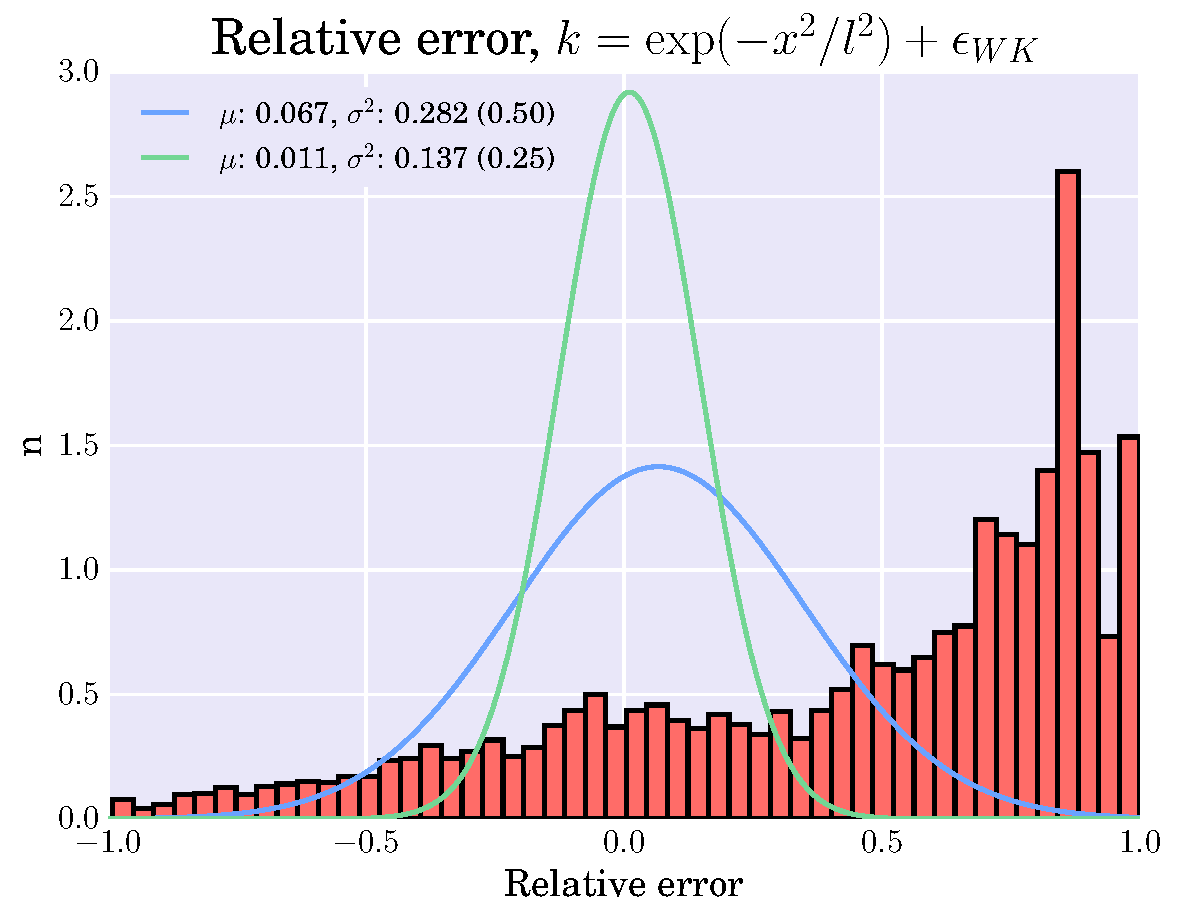
\includegraphics[scale=0.5]{/home/ingrid/Documents/Master/ML/Abel_lin_log_20000/plots/errors_k4_05.pdf}
\caption{Normalized histogram of relative errors $(y_{true} - y_{predict})/y_{true}$ for 1000 training points and 10000 test points run on Abel supercluster. Input parameters are $m_{\tilde{g}}$ and $m_{\tilde{c}_L}$. A Gaussian curve has been fitted using $scipy.stats.norm$.}
\label{Fig:: Abel 20000p 0.5 k4 errors with gaussian fit}
\end{figure}


The array of errors is evaluated, and values outside of given limits $ [-lim, lim ] $ are removed. Then a Gaussian is fitted, with the goal of reaching $\sigma^2 \leq 10 \%$. For $lim=0.25$ the fraction of removed points is $0.1879$, which yields a Gaussian approximation with $\mu = -0.010$ and $\sigma^2 = 0.107$, as can be seen in Fig. (\ref{Fig:: Abel 20000p errors cut with gaussian fit}).


\begin{figure}[H]
\centering
\includegraphics[scale=0.5]{/home/ingrid/Documents/Master/ML/Abel_lin_log_20000/Plots/errors_split_data.pdf}
\caption{Normalized histograms for decades of $\log (NLO)$. 10000 training points and 10 000 test points run on Abel supercluster. Input parameters are $m_{\tilde{g}}$ and $m_{\tilde{c}_L}$.}
\label{Fig:: Abel 20000p histograms of decades}
\end{figure}



A comparison of the number of points and kernels used is found in Tab. ().

\begin{table}
\centering
\begin{tabular}{ccccccc}
\toprule
Training fraction &  \multicolumn{3}{c}{$[-0.5, 0.5]$} & \multicolumn{3}{c}{$[-0.25,0.25]$}\\
\midrule
{}  & $\mu$ & $\sigma^2$ & $n/N$ & $\mu$ & $\sigma^2$ & $n/N$\\
0.001 & 0.08461 & 0.28602 & 0.9657 & 0.03074 & 0.14497 & 0.9836\\
0.01 & 0.04682 & 0.28424 & 0.5857 & 0.01186 & 0.14657 & 0.7996\\
0.1 \\
0.5 & -0.01720 & 0.16024 & 0.0682 & -0.01030 & \color{red}{0.10699} & 0.1879\\
\bottomrule
\end{tabular}
\caption{Gaussian fit parameters for the 20 000 point Gaussian Process approximations, using kernel 4 ($k = \exp (-x^2/\ell^2) + \epsilon_{WK}$). The parameter $n/N$ is the fraction of test points that lies outside the given interval.}
\label{Tab:: GP 20k comparison of training fractions k4}
\end{table}

\begin{table}
\centering
\begin{tabular}{ccccccc}
\toprule
Training fraction &  \multicolumn{3}{c}{$[-0.5, 0.5]$} & \multicolumn{3}{c}{$[-0.25,0.25]$}\\
\midrule
{}  & $\mu$ & $\sigma^2$ & $n/N$ & $\mu$ & $\sigma^2$ & $n/N$\\
0.01 & 0.03839 & 0.26943 & 0.8008 & 0.01303 & 0.14037 & 0.8915\\
0.1 & 0.03689 & 0.26431 & 0.7792 & 0.01288 & 0.14055 & 0.8730\\
0.5 & 0.02760 & 0.26557 & 0.7273 & 0.00545 & 0.13901 & 0.8425\\
\bottomrule
\end{tabular}
\caption{Gaussian fit parameters for the 20 000 point Gaussian Process approximations, using kernel 1 ($k = C \exp (-x^2/\ell^2)$, where $C$ is a constant). The parameter $n/N$ is the fraction of test points that lies outside the given interval.}
\label{Tab:: GP 20k comparison of training fractions k1}
\end{table}

\begin{table}
\centering
\begin{tabular}{ccccccc}
\toprule
Training fraction &  \multicolumn{3}{c}{$[-0.5, 0.5]$} & \multicolumn{3}{c}{$[-0.25,0.25]$}\\
\midrule
{}  & $\mu$ & $\sigma^2$ & $n/N$ & $\mu$ & $\sigma^2$ & $n/N$\\
0.01 & -0.02114 & 0.19631 & 0.2023 & 0.00143 & 0.12699 & 0.3651\\
0.1 & -0.01882 & 0.16521 & 0.0669 & -0.01110 & 0.11044 & 0.1961\\
0.5 & -0.02015 & 0.15642 & 0.0574 & -0.01270 & \color{red}{0.10524} & 0.1707\\
\bottomrule
\end{tabular}
\caption{Gaussian fit parameters for the 20 000 point Gaussian Process approximations, using kernel 5 ($k = C \exp (-x^2/\ell^2) + \epsilon_{WK}$, where $C$ is a constant). The parameter $n/N$ is the fraction of test points that lies outside the given interval.}
\label{Tab:: GP 20k comparison of training fractions k5}
\end{table}



\pagebreak

Testing kernels of Abel.



\begin{table}[H]
\centering
\begin{tabular}{|c|l|}
\hline
Kernel & Specifics\\
\hline
1 & $C(1.0, (1e-2, 1e2)) * RBF(10, (1e-3, 1e3))$\\
\hline
2 & $DotProduct(sigma\_0=1.0, sigma\_0\_bounds=(1e-05, 100.0))$\\
\hline
3 & $ExpSineSquared(length\_scale=10.0, periodicity=1.0,$\\
&$ length\_scale\_bounds=(1e-02, 1000.0), periodicity\_bounds=(1e-02, 1000.0))$\\
\hline
4 & $RBF(936, (1e-2, 1e5))$\\
&$ + WhiteKernel(noise\_level=0.374, noise\_level\_bounds=(1e-10, 1e+2))$\\
\hline
\end{tabular}
\end{table}

\begin{table}[H]
\begin{tabular}{|c|l|l|l|l|}
\hline
Kernel & Fraction & Optimized kernel & $\mu$ & $\sigma$\\
\hline
1 & 0.1665 & $C = 10**2$, $length\_scale=833$ & -0.02154 & 0.19508\\
2 & 0.7988 & $sigma\_0=2.01$ & 0.05088 & 0.29124\\
3 & NA\\
4 & 0.7480 & $length\_scale=2.44e+03$, $ noise\_level=1.78$ & 0.03848 & 0.28073\\
\hline
\end{tabular}
\end{table}


%Error histograms for different kernels

\begin{figure}
\centering
	\begin{subfigure}[b]{0.65\textwidth}
	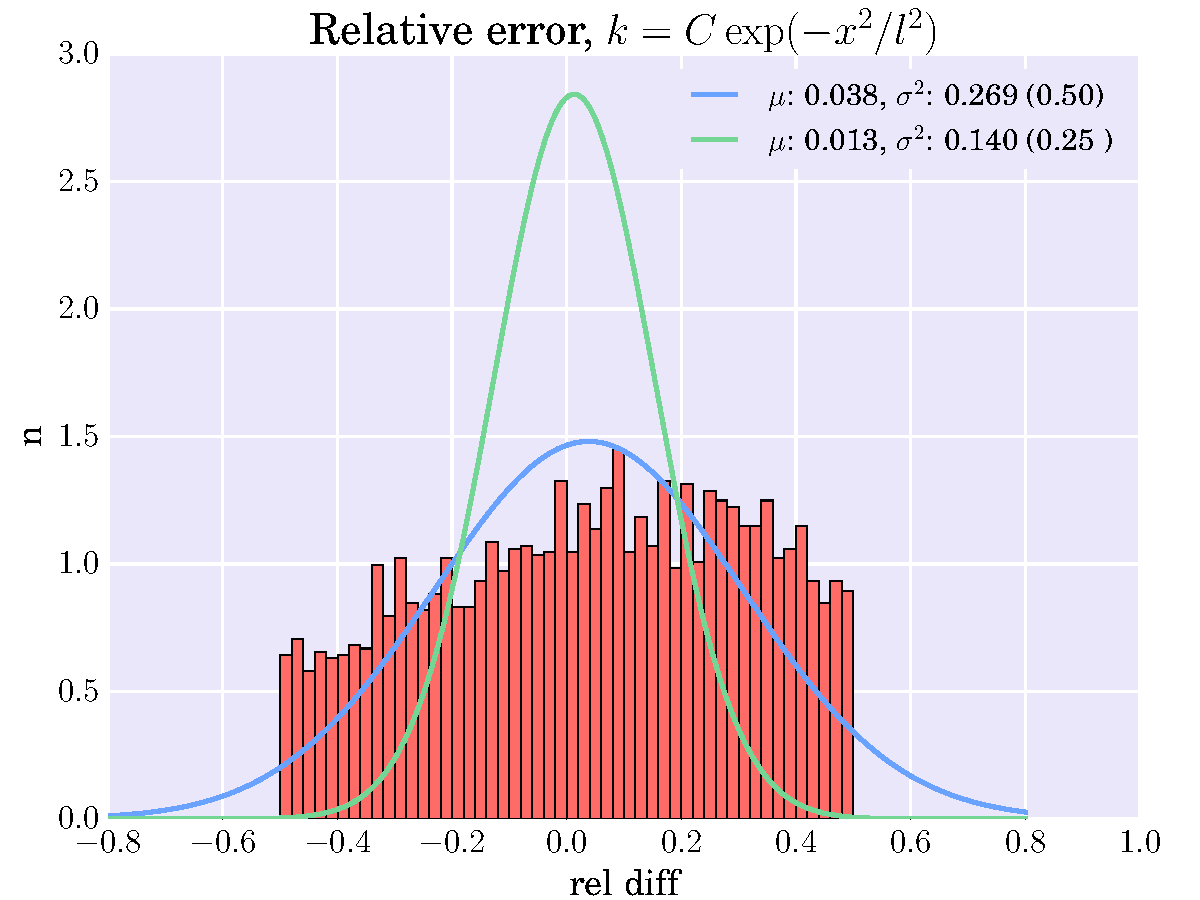
\includegraphics[width=\textwidth]{/home/ingrid/Documents/Master/ML/Abel_lin_log_20000/plots/errors_k1_001.pdf}
	\caption{Training fraction 0.01.}
	\end{subfigure}
	\begin{subfigure}[b]{0.65\textwidth}
	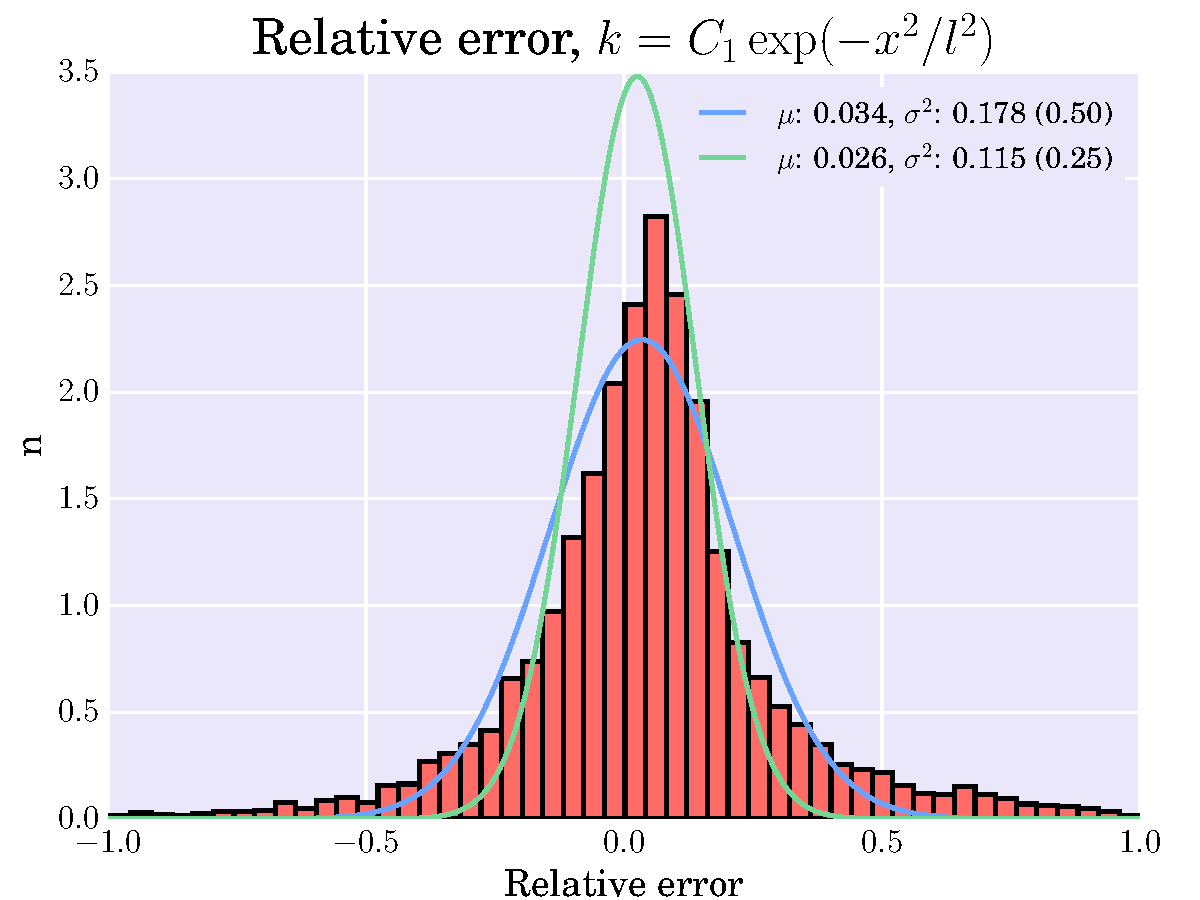
\includegraphics[width=\textwidth]{/home/ingrid/Documents/Master/ML/Abel_lin_log_20000/plots/errors_k1_01.pdf}
	\caption{Training fraction 0.1.}
	\end{subfigure}
	\begin{subfigure}[b]{0.65\textwidth}
	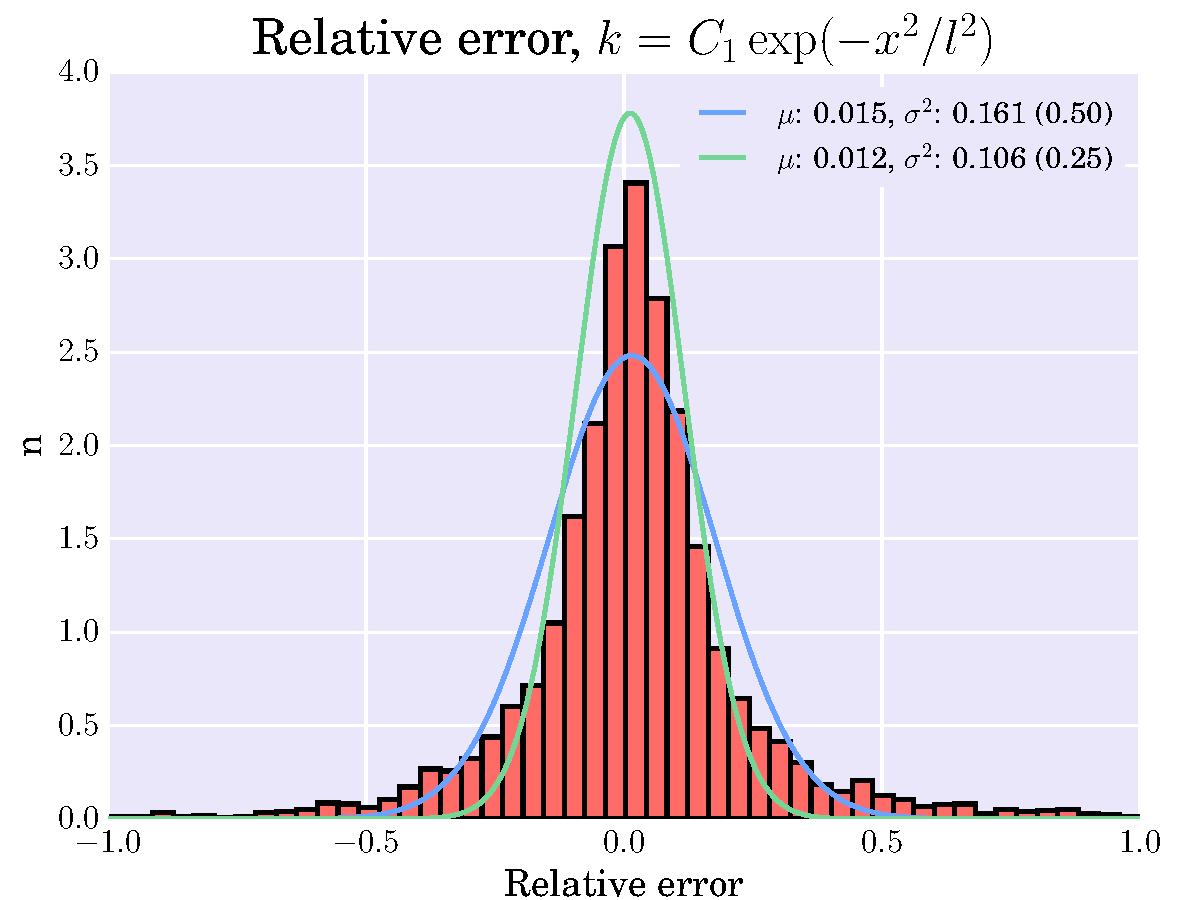
\includegraphics[width=\textwidth]{/home/ingrid/Documents/Master/ML/Abel_lin_log_20000/plots/errors_k1_05.pdf}
	\caption{Training fraction 0.5.}
	\end{subfigure}
\caption{Normalized histogram of relative errors $(y_{true} - y_{predict})/y_{true}$ for 20000 training points run on Abel supercluster, with kernel $kernel1 = C \exp(-x^2/\ell^2)$. Input parameters are $m_{\tilde{g}}$ and $m_{\tilde{c}_L}$. A Gaussian curve has been fitted using $scipy.stats.norm$.}
\label{Fig:: Error histograms k1 abel 20k}
\end{figure}


\begin{figure}
\centering
	\begin{subfigure}[b]{0.65\textwidth}
	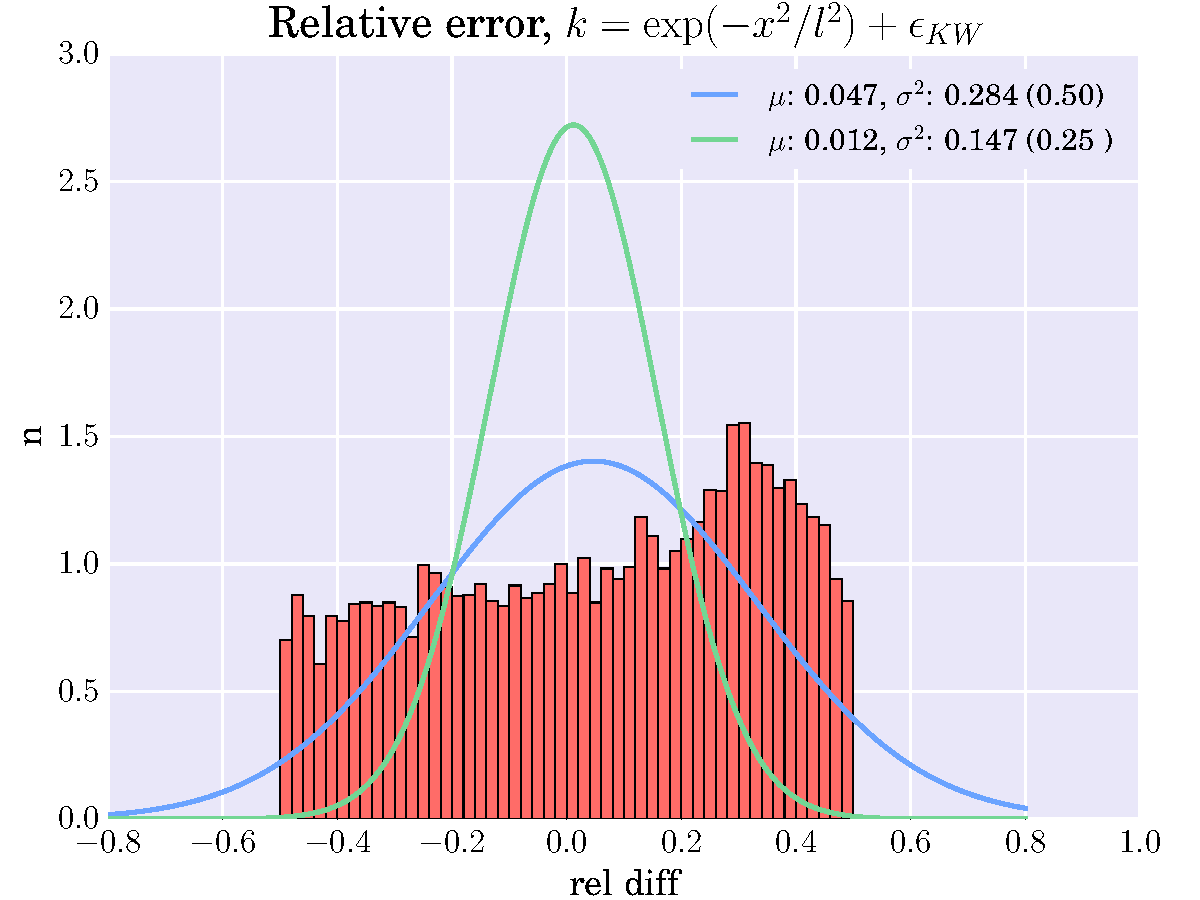
\includegraphics[width=\textwidth]{/home/ingrid/Documents/Master/ML/Abel_lin_log_20000/plots/errors_k4_001.pdf}
	\caption{Training fraction 0.01.}
	\end{subfigure}
	\begin{subfigure}[b]{0.65\textwidth}
	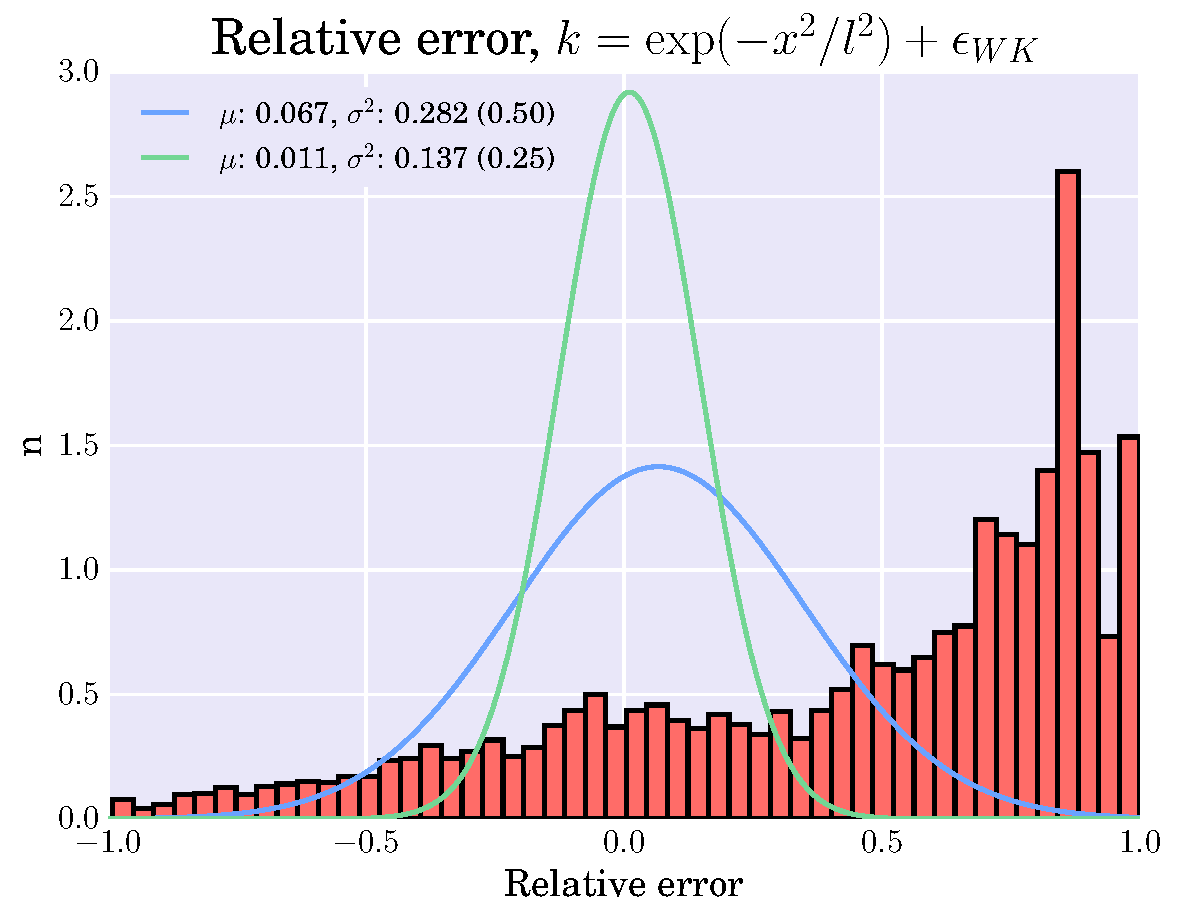
\includegraphics[width=\textwidth]{/home/ingrid/Documents/Master/ML/Abel_lin_log_20000/plots/errors_k4_05.pdf}
	\caption{Training fraction 0.5.}
	\end{subfigure}
\caption{Normalized histogram of relative errors $(y_{true} - y_{predict})/y_{true}$ for 20000 training points run on Abel supercluster, with kernel $kernel4 = \exp(-x^2/\ell^2) + \epsilon_{WK}$. Input parameters are $m_{\tilde{g}}$ and $m_{\tilde{c}_L}$. A Gaussian curve has been fitted using $scipy.stats.norm$.}
\label{Fig:: Error histograms k4 abel 20k}
\end{figure}

\begin{figure}
\centering
	\begin{subfigure}[b]{0.65\textwidth}
	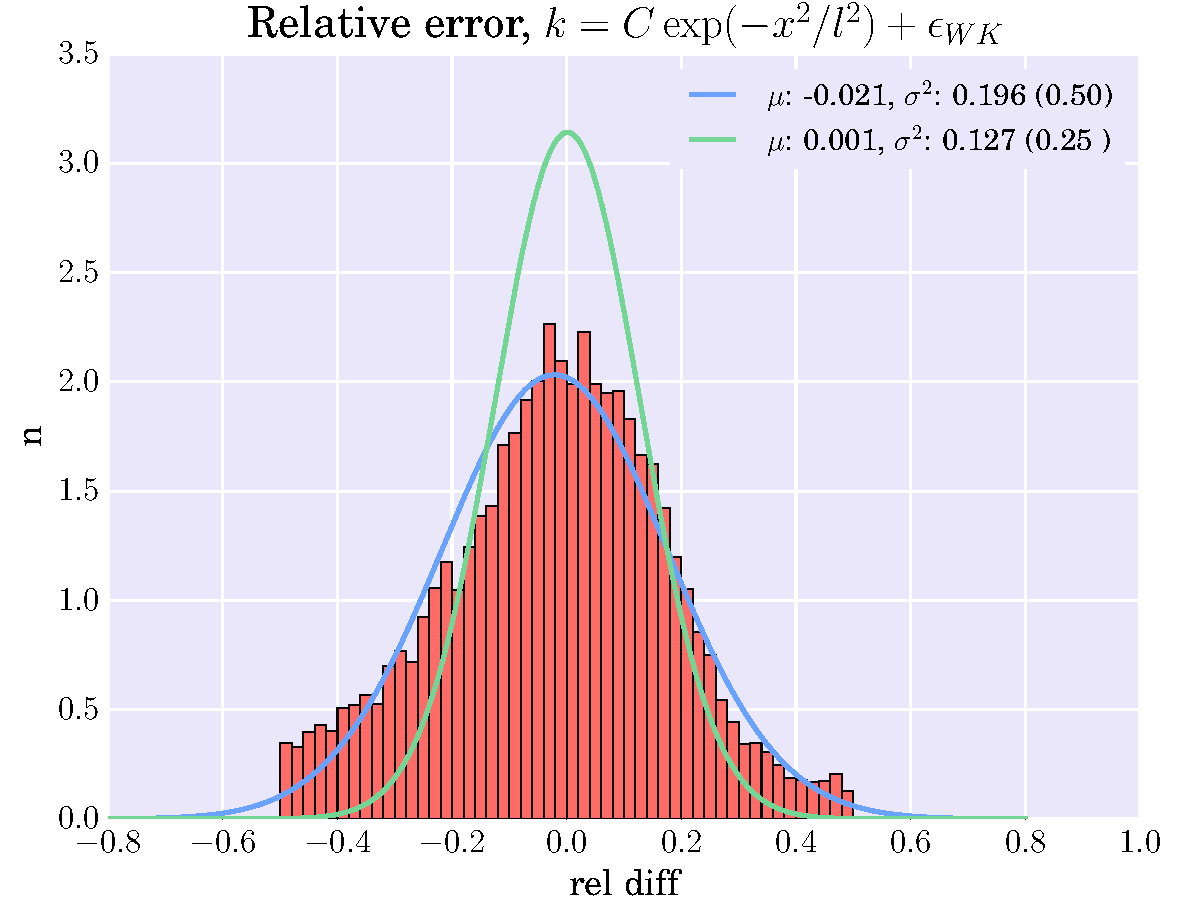
\includegraphics[width=\textwidth]{/home/ingrid/Documents/Master/ML/Abel_lin_log_20000/plots/errors_k5_001.pdf}
	\caption{Training fraction 0.01.}
	\end{subfigure}
	\begin{subfigure}[b]{0.65\textwidth}
	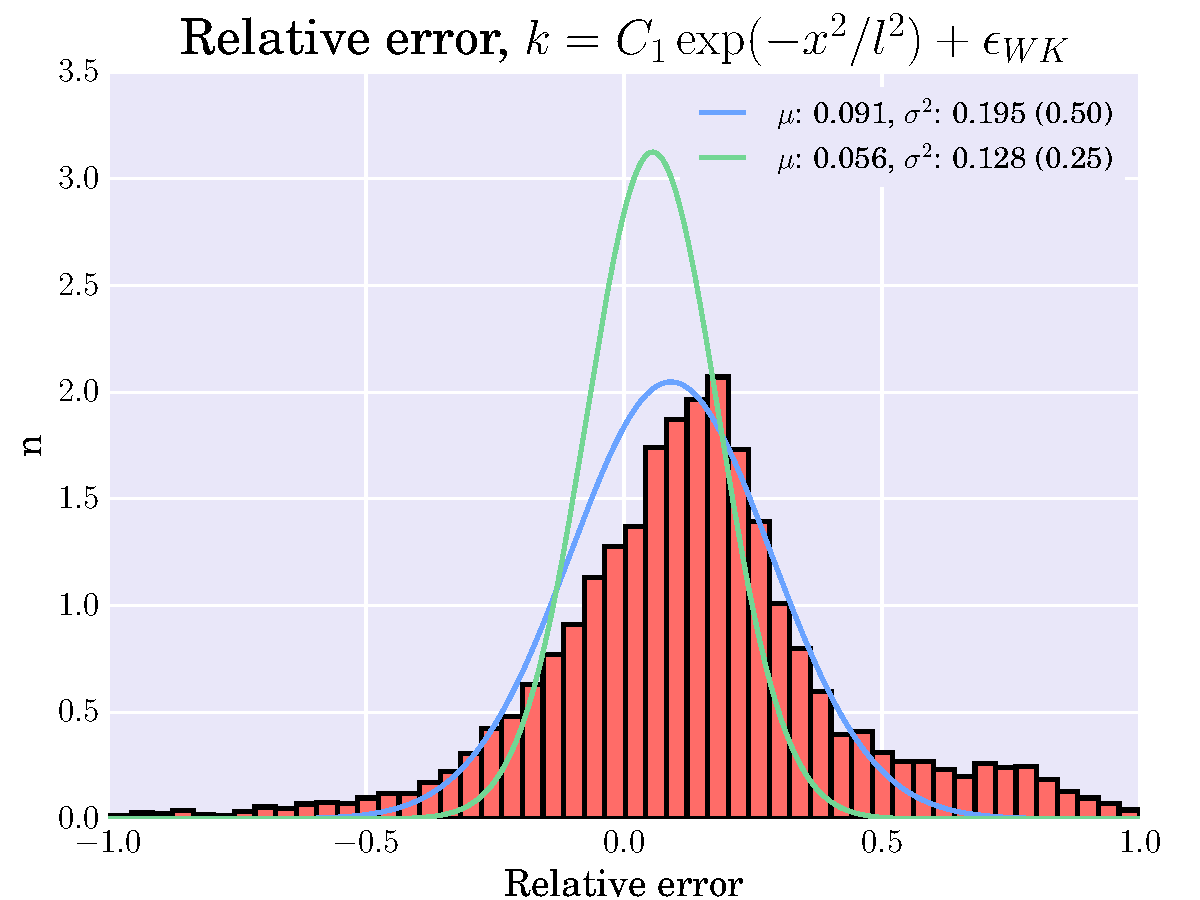
\includegraphics[width=\textwidth]{/home/ingrid/Documents/Master/ML/Abel_lin_log_20000/plots/errors_k5_01.pdf}
	\caption{Training fraction 0.1.}
	\end{subfigure}
	\begin{subfigure}[b]{0.65\textwidth}
	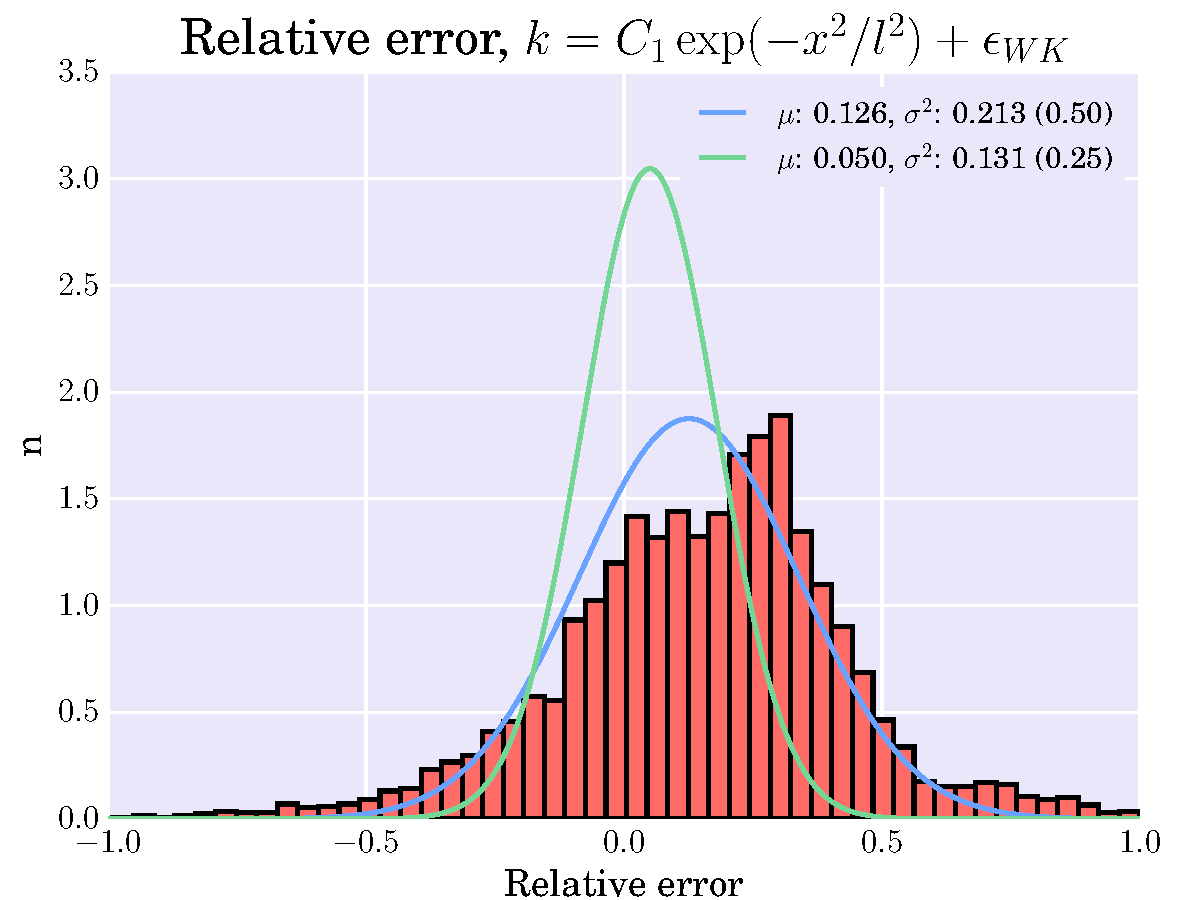
\includegraphics[width=\textwidth]{/home/ingrid/Documents/Master/ML/Abel_lin_log_20000/plots/errors_k5_05.pdf}
	\caption{Training fraction 0.5.}
	\end{subfigure}
\caption{Normalized histogram of relative errors $(y_{true} - y_{predict})/y_{true}$ for 20000 training points run on Abel supercluster, with kernel $kernel5 = C \exp(-x^2/\ell^2)+ \epsilon_{WK}$. Input parameters are $m_{\tilde{g}}$ and $m_{\tilde{c}_L}$. A Gaussian curve has been fitted using $scipy.stats.norm$.}
\label{Fig:: Error histograms k5 abel 20k}
\end{figure}


Comparing mean and std.

\begin{figure}[H]
\centering
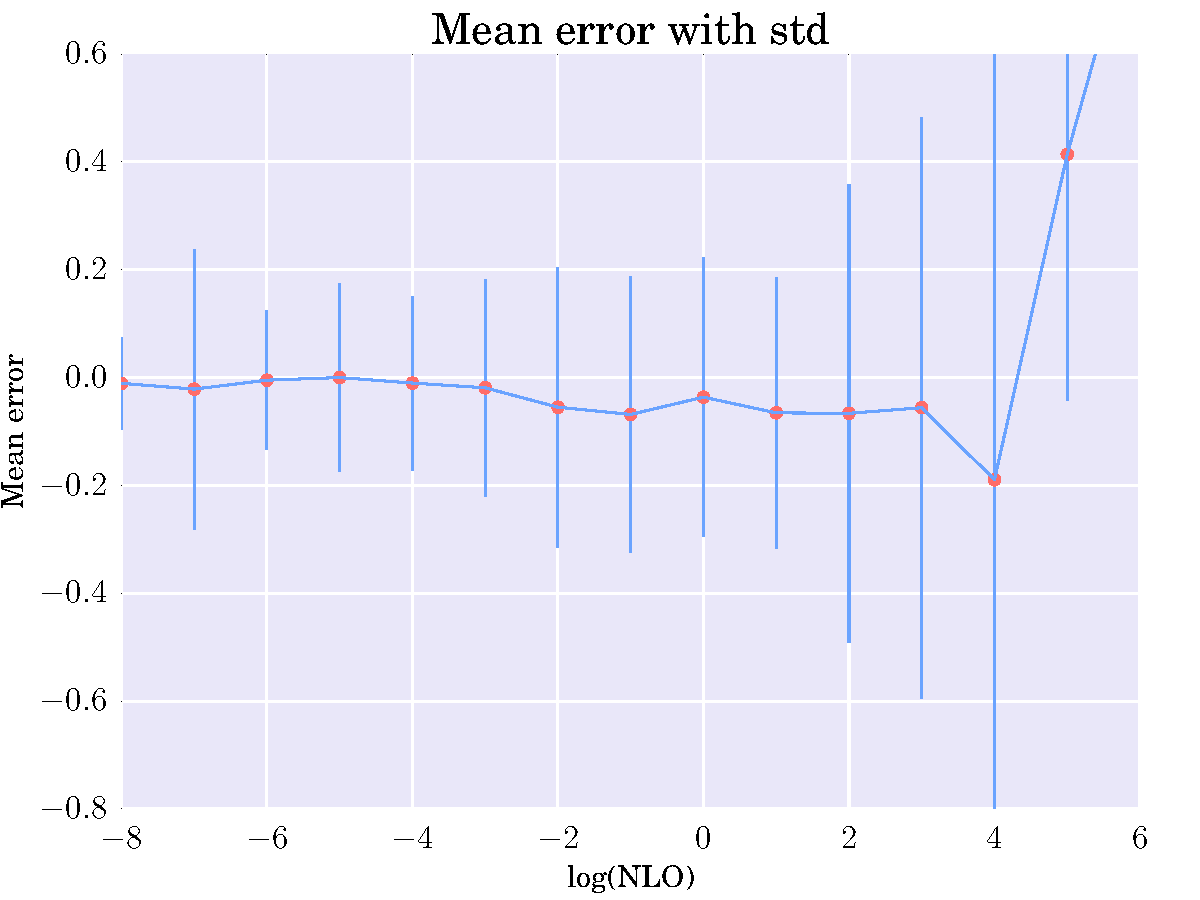
\includegraphics[scale=0.5]{/home/ingrid/Documents/Master/ML/Abel_lin_log_20000/plots/mean_sigma_k4_05.pdf}
\caption{Mean error with standard deviation as a function of $\log (NLO)$. Values less than $-7$ are not considered, as the luminosity at the LHC is $30$ fb$^{-1}$, and so smaller cross sections give $<1$ detectable particles. 10 000 training points and 10 000 test points run on Abel supercluster, with kernel $kernel4 = \exp(-x^2/\ell^2) + \epsilon_{WK}$. Input parameters are $m_{\tilde{g}}$ and $m_{\tilde{c}_L}$.}
\end{figure}

\begin{figure}[H]
\centering
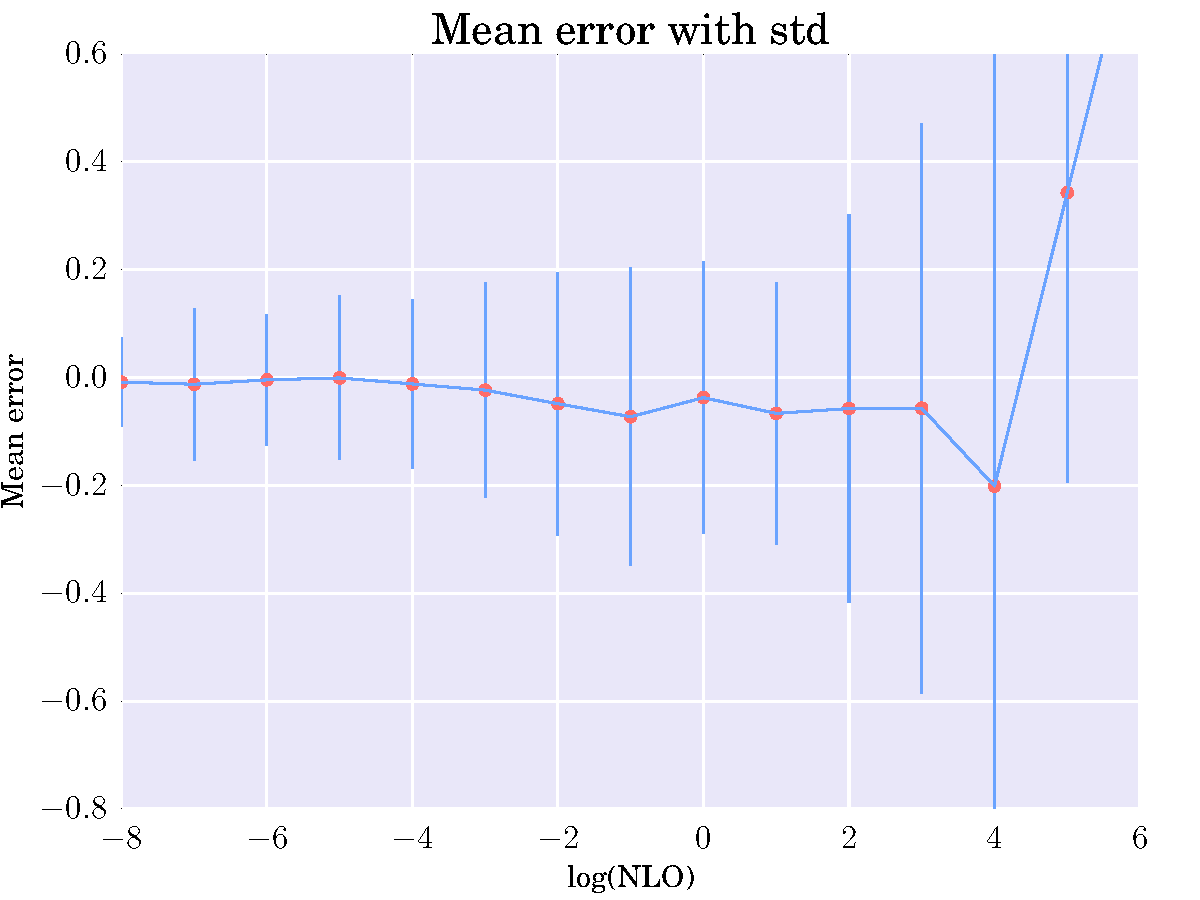
\includegraphics[scale=0.5]{/home/ingrid/Documents/Master/ML/Abel_lin_log_20000/plots/mean_sigma_k5_05.pdf}
\caption{Mean error with standard deviation as a function of $\log (NLO)$. Values less than $-7$ are not considered, as the luminosity at the LHC is $30$ fb$^{-1}$, and so smaller cross sections give $<1$ detectable particles. 10000 training points and 10 000 test points run on Abel supercluster with kernel $kernel5 = C\exp(-x^2/\ell^2) + \epsilon_{WK}$. Input parameters are $m_{\tilde{g}}$ and $m_{\tilde{c}_L}$.}
\end{figure}











\end{document}